\chapter{Fundamentals}
\label{sec:fundamentals}

% \begin{itemize}
% 	\item describe methods and techniques that build the basis of your work
% 	\todo{don't get what methods and techniques i was using}
% 	\item include what's needed to understand your work (e.g., techniques, protocols, models, hardware, software, ...)
% 	\item exclude what's not (e.g., anything you yourself did, anything your reader can be expected to know, ...)
% 	\item review related work(!)
% 	\item recommended length: approximately one third of the thesis.
% \end{itemize}

In this chapter explains the fundamentals required for understanding the different approaches 
in this thesis.
This contains basic knowledge of the physical- and data link layer,
which are located in the first and second layer of the \ac{OSI} Model.

It also explains what types of transmissions exist, 
introduces the hardware used in this thesis and explains the ESP-NOW protocol running on this hardware.

\begin{table}[h]
	\centering
	% \label{tab:layer_overview}
	\begin{tabular}{ |c| } 
		\hline
		Application layer\\
		\hline
		Presentation layer\\
		\hline
		Session layer\\
		\hline
		Network layer\\
		\hline
		\cellcolor{yellow!25}Data Link layer\\
		\hline
		\cellcolor{yellow!25}Physical layer\\
		\hline
	\end{tabular}
	\caption{\ac{OSI} model}
	\label{tab:OSI}
\end{table}

\section{IEEE 802.11 Protocol}

The \ac{IEEE} 802 is a family of standards dealing with area networks of different kinds.
\begin{itemize}
	\item 802.11 \ac{WLAN}
	\item 802.15.1 Wireless Personal Area Network (WPAN)
	\item 802.15.4 Low-rate WPAN (LR-WPAN)
	\item 802.16 Wireless metropolitan area network (WMAN)
\end{itemize}

For this thesis is the focus set to the 802.11, because of the accessability and wide functionality.
There are two \ac{BSS} defined:
\begin{itemize}
	\label{itm:bss}
	\item Infrastructure BSS\\
	A central element manages the network and all the traffic goes through. 
	Every \ac{STA} must always communicate via the \ac{AP} and never directly - exceptional: Direct Link Mode.
	An initial association must take place to use the Infrastructure \ac{BSS}.
	
	\item Independent BSS\\
	A network without a central station, where the network topology can flexibly change over time.
	The communication happens directly between the Wireless Endsystems.
	Efficent routing can become a problem in more complex topologys.
\end{itemize}
The most common use in 802.11 is the Infrastructure mode, which is commonly used in office and home enviroments.\\ 

\subsection*{Physical layer}

In this thesis a brief look into the Physical Network Layer (PHY) of the IEEE 802.11 standard, 
which is the first layer of the OSI model \ref{tab:OSI}, should be taken.
This layer provides mechanical, electrical and other functional tools to activate or deactivate physical connections, maintain them and transmit bits over them. 
These can be, for example, electrical signals, optical signals (fiber optics, lasers) or electromagnetic waves (wireless networks).
There are several complements to the 802.11 standard, the most common are:

\begin{itemize}
	\item 802.11b \\
	Supports larger bitrates with \ac{DSSS} or \ac{FHSS} as modulation from 1Mbps to 11Mbbps.
	It uses the 2.4 GHz ISM band.
	\item 802.11a and 802.11g \\
	With \ac{OFDM} data rates is increased by up to 54 Mbps.
	Where 802.11a is in the 5GHz ISM band 802.11g uses the 2.4GHz ISM band.
	\item 802.11n\\
	It also uses \ac{OFDM} and improves with additionaly \ac{MIMO}, channel bonding and frame aggregation to increase the bandwidth and decrease the overhead.
	Using 2.4 GHz and 5GHz ISM band.
	\item 802.11ac\\
	Support of wider channel and out of it higher bitrates. It also includes features like Multi-User MIMO.
	It only uses the 5 GHz ISM band.
	\item 802.11ax\\
	Like 802.11ac but with additional use of the 6GHz ISM band and better power control. 
	Also called WiFi6.
\end{itemize}

There are a few more specifications, in this thesis the rather basic 802.11b is used with a transmission rate of 1Mbps.

\subsection*{Data Link Layer}

The \ac{DL} Layer is the second-lowest layer of the \ac{OSI} Model \ref{tab:OSI} and is split into two sublayers. 
The \ac{LLC} sublayer which multiplex protocols over the MAC layer while transmitting and to de-multiplex the protocols while receiving.
LLC provides the hop-to-hop flow and error control, allows multipoint communication over networks 
and adds frame sequence numbers.
But thesis focuses on the other data link sublayer.

The \ac{MAC} is the second sublayer and 
includes network protocols that regulate how multiple computers share the physical transmission medium they use. 
Without regulation, collisions and data loss would occur in the shared medium if several stations were to transmit simultaneously.
The \ac{MAC} Protocol Data Unit is aditionally added inside the \ac{PHY} Payload. 
It contains the \ac{MAC} Header and encapsulated in it the \ac{MSDU}.

\begin{figure}[h]
	\centering
	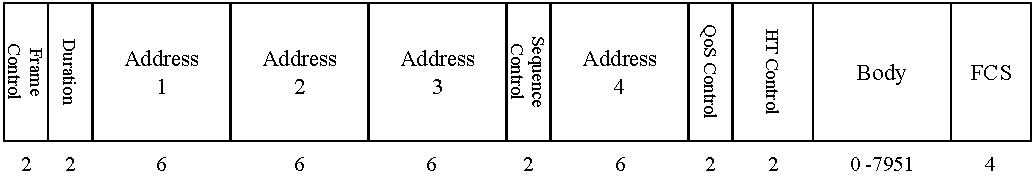
\includegraphics[scale=0.67]{figures/MACFrame.pdf}
	\label{fig:mac_header}
	\caption{Mac Frame Header}
\end{figure}

\begin{itemize}
	\setlength\itemsep{-0.0em}
	\item \textbf{Frame Control Field:} Discribes the Type of frame:
	\begin{itemize}
		\setlength\itemsep{-0.0em}
		\item 00 Manegement Frame
		\item 01 Control Frame
		\item 10 Data Frame
	\end{itemize}
	\item \textbf{Duration:} Contains the \ac{NAV} value, specifies the transmission time required for the frame. 
	In order to save energy, stations can defer access to the medium for the given duration.
	\item \textbf{Address fields:} Certain address fields are specified by the relative position of the address field.
	Not every address field is needed by certain frames. Each device is associated with a unique \ac{MAC} address.
	\begin{itemize}
		\setlength\itemsep{-0.0em}
		\item \ac{BSSID}
		\item Source Address
		\item Destination Address
		\item Transmitting STA Address
		\item Receiving STA Address
	\end{itemize}
	\item \textbf{Sequence Control:} Sequence number of the current frame modulo 4096.
	\item \textbf{MAC Body:} The actual payload information of the \ac{MAC} layer. 
	The actual payload can differ, because the headers of the \ac{LLC} and ip etc. has to be subtracted.
	\item \textbf{QoS Control:} Identifies the Quality of Service parameter of the data frame
	\item \textbf{Frame Check Frequence:} The sender calculates the checksum for the entire data block and appends it to the end of the block.
\end{itemize}

\subsection*{Carrier Sense Multiple Access/Collision Avoidance}

\ac{CSMA/CA} is composed of:
\begin{itemize}
	\setlength\itemsep{-0.0em}
	\item \textbf{CS (Carrier Sense):} Each station checks whether the medium is free before transmitting
	\item \textbf{MA (Multiple Access)}: Several stations share one medium, which can also be a cable.
	\item \textbf{CD (Collision Detection):} A schedule prevents two stations from starting their transmission at the same time.
\end{itemize}

\begin{figure}[h]
	\centering
	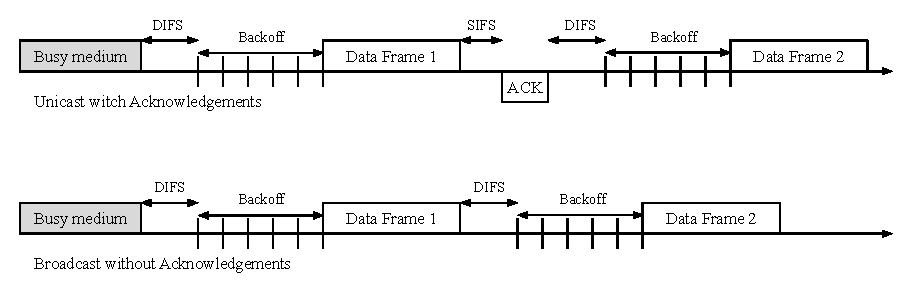
\includegraphics[scale=0.75]{figures/CSMA_CD.pdf}
	\caption{CSMA/CA with and without acknowledgements}
	\label{fig:CSMACD}
\end{figure}

Before a station transmitts data it has to check or listen to the medium to avoid collision resulting in packet loss.
Only when the medium is free, the station waits for a \ac{DIFS} and a random backoff.
The backoff is a random time within a \ac{CW} to prevent all stations from transmitting immediately after the \ac{DIFS}.
The \ac{CW} consists of several slots, each consisting of 20$\mu$s in 802.11b.
If a transmission was not successful, the station doubles the \ac{CW}, 
this doubles the average waiting time and is intended to prevent re-collisions.
The minimum \ac{CW} in 802.11b is set to 16 slots.
Before sending an acknowledgement, the station only waits for a \ac{SIFS}, 
which is significantly shorter than the \ac{DIFS} because the acknowledgement frame is prioritised before the next frame.

\subsection*{Data Link Transmissions}

When packets are sent on the data link layer, they do not contain the headers to the layers above, such as TCP/IP.
Therefore, IP addresses cannot be used to transmit packets to another network.
There are three basic types of data link transmissions: unicast, broadcast and multicast.

\subsubsection*{Unicast}
\label{sec:unicast}

The link layer unicast is used to sent data over a single hop to the target \ac{WES} destination.
The link layer of each \ac{WES} checks the destination MAC address in the link layer header and 
discards the frame if the destination address does not match its own address.
It is therefore a direct communication between the transmitter and the WES.

Unicast is by default reliable.
When the Unicast reaches the destination \ac{WES} without missing or broken bytes 
an acknowledgement frame is send back after the \ac{SIFS}.
If the acknowledgement is not successfully received by the sender, the sender will repeat the transmission for a given number.
When the number is exceeded, the packet could not be delivered. 
If the number is set to zero, the unicast can be considered as non-reliable.
After each unsuccessful delivery, the size of the \ac{CW} is doubled.

\begin{figure}[h]
	\centering
	\begin{tikzpicture}[node distance={10mm}, main/.style = {draw, circle}] 
		\node[main] (1) 							{TX}; 
		\node[main] (2) [right=0cm and 2cm of 1]	{$\text{RX}_2$}; 
		\node[main] (3) [above of =2]				{$\text{RX}_1$}; 
		\node[main] (4) [below of =2]				{$\text{RX}_3$}; 
		\draw[->] (1) -- (2);
	\end{tikzpicture} 
	\caption{Unicast Transmission}
	\label{fig:unicast_topology}
\end{figure}

\subsubsection*{Broadcast}
\label{sec:DLbroadcast}

If a packet should be received from all \ac{WES}s it can be distributed as a broadcast,
while setting the \ac{MAC} address of the destination address in the link layer to the common broadcast address, which is ff:ff:ff:ff:ff:ff.

In contrast to unicast, broadcast is not reliable. 
This is mainly because the packet is addressed to all nodes at the same time, 
and if link layer acknowledgements would be used, 
the acknowledgements would be sent by all nodes at the same time, 
because there is no mechanism in which order acknowledges should be answered. 
Retransmitting all acknowledgements at the same time would lead to massive 
collision and loss of acknowledgements.
In addition, the sender of a broadcast does not know how many WESs he is addressing the packet to in the 
first place.

For example, in a \ac{WLAN} management information is sent as a broadcast,
because it has to reach every station and isn't worth to be acknowleged.

\begin{figure}[h]
	\centering
	\begin{tikzpicture}[node distance={10mm}, main/.style = {draw, circle}] 
		\node[main] (1) 							{TX}; 
		\node[main] (2) [right=0cm and 2cm of 1]	{$\text{RX}_2$}; 
		\node[main] (3) [above of =2]				{$\text{RX}_1$}; 
		\node[main] (4) [below of =2]				{$\text{RX}_3$}; 
		\draw[->] (1) -- (2);
		\draw[->] (1) -- (3);
		\draw[->] (1) -- (4);
	\end{tikzpicture} 
	\caption{Broadcast Transmission}
	\label{fig:broadcast_topology}
\end{figure}

\subsubsection*{Multicast}

When the same packet should be transmitted to multiple \ac{WES}s, but not to all, multicast can be used.
Transmitting the same packet multiple times via unicast is wasteful.
For this purpose, there is a corresponding multicast addresses. 
They exist only as destination addresses.

With multicast, the use of acknowledgements is possible because the sender knows how many receivers there are.
There are different approaches to realize acknowledgements for mutlicasts, 
they differ mainly by the respective field of application,
an approach for robust multicast in video transmissions is given by Mihaela van der Schaar et al. in \cite{EvaluationOfErrorControl}.
Level 2 multicast is often used for large files in audio or video streams, 
where a big amount of data is distributed and multiple clients listen simultaneously.

\begin{figure}[h]
	\centering
	\begin{tikzpicture}[node distance={10mm}, main/.style = {draw, circle}] 
		\node[main] (1) 							{TX}; 
		\node[main] (2) [right=0cm and 2cm of 1]	{$\text{RX}_2$}; 
		\node[main] (3) [above of =2]				{$\text{RX}_1$}; 
		\node[main] (4) [below of =2]				{$\text{RX}_3$}; 
		\draw[->] (1) -- (2);
		\draw[->] (1) -- (4);
	\end{tikzpicture} 
	\caption{Multicast Transmission}
	\label{fig:multicast_topology}
\end{figure}

\section{Light protocols}

There are several lighting protocols that are used. The field of application ranges from wired CAN buses over ethernet cables to wireless WLAN networks.
To give a short insight, some of the most important protocols are explained below.

\subsection*{DMX-512a}
\ac{DMX} 512a, is the current industry standard for stage lighting. It is based on \ac{CANproto}, therefore it uses wires.
Physically is the DMX protocol is transmitted over a differential pair of lines using the RS-485 voltage levels. 
The bus signal is updated with 44Hz.
According to the specification XLR-5 type connectors are to be used (\cref{fig:xlr}\footnote{Image available at \url{https://upload.wikimedia.org/wikipedia/commons/thumb/1/1c/XLR5_pinouts.svg/2560px-XLR5_pinouts.svg.png}}).

\begin{figure}[h]
	\centering
	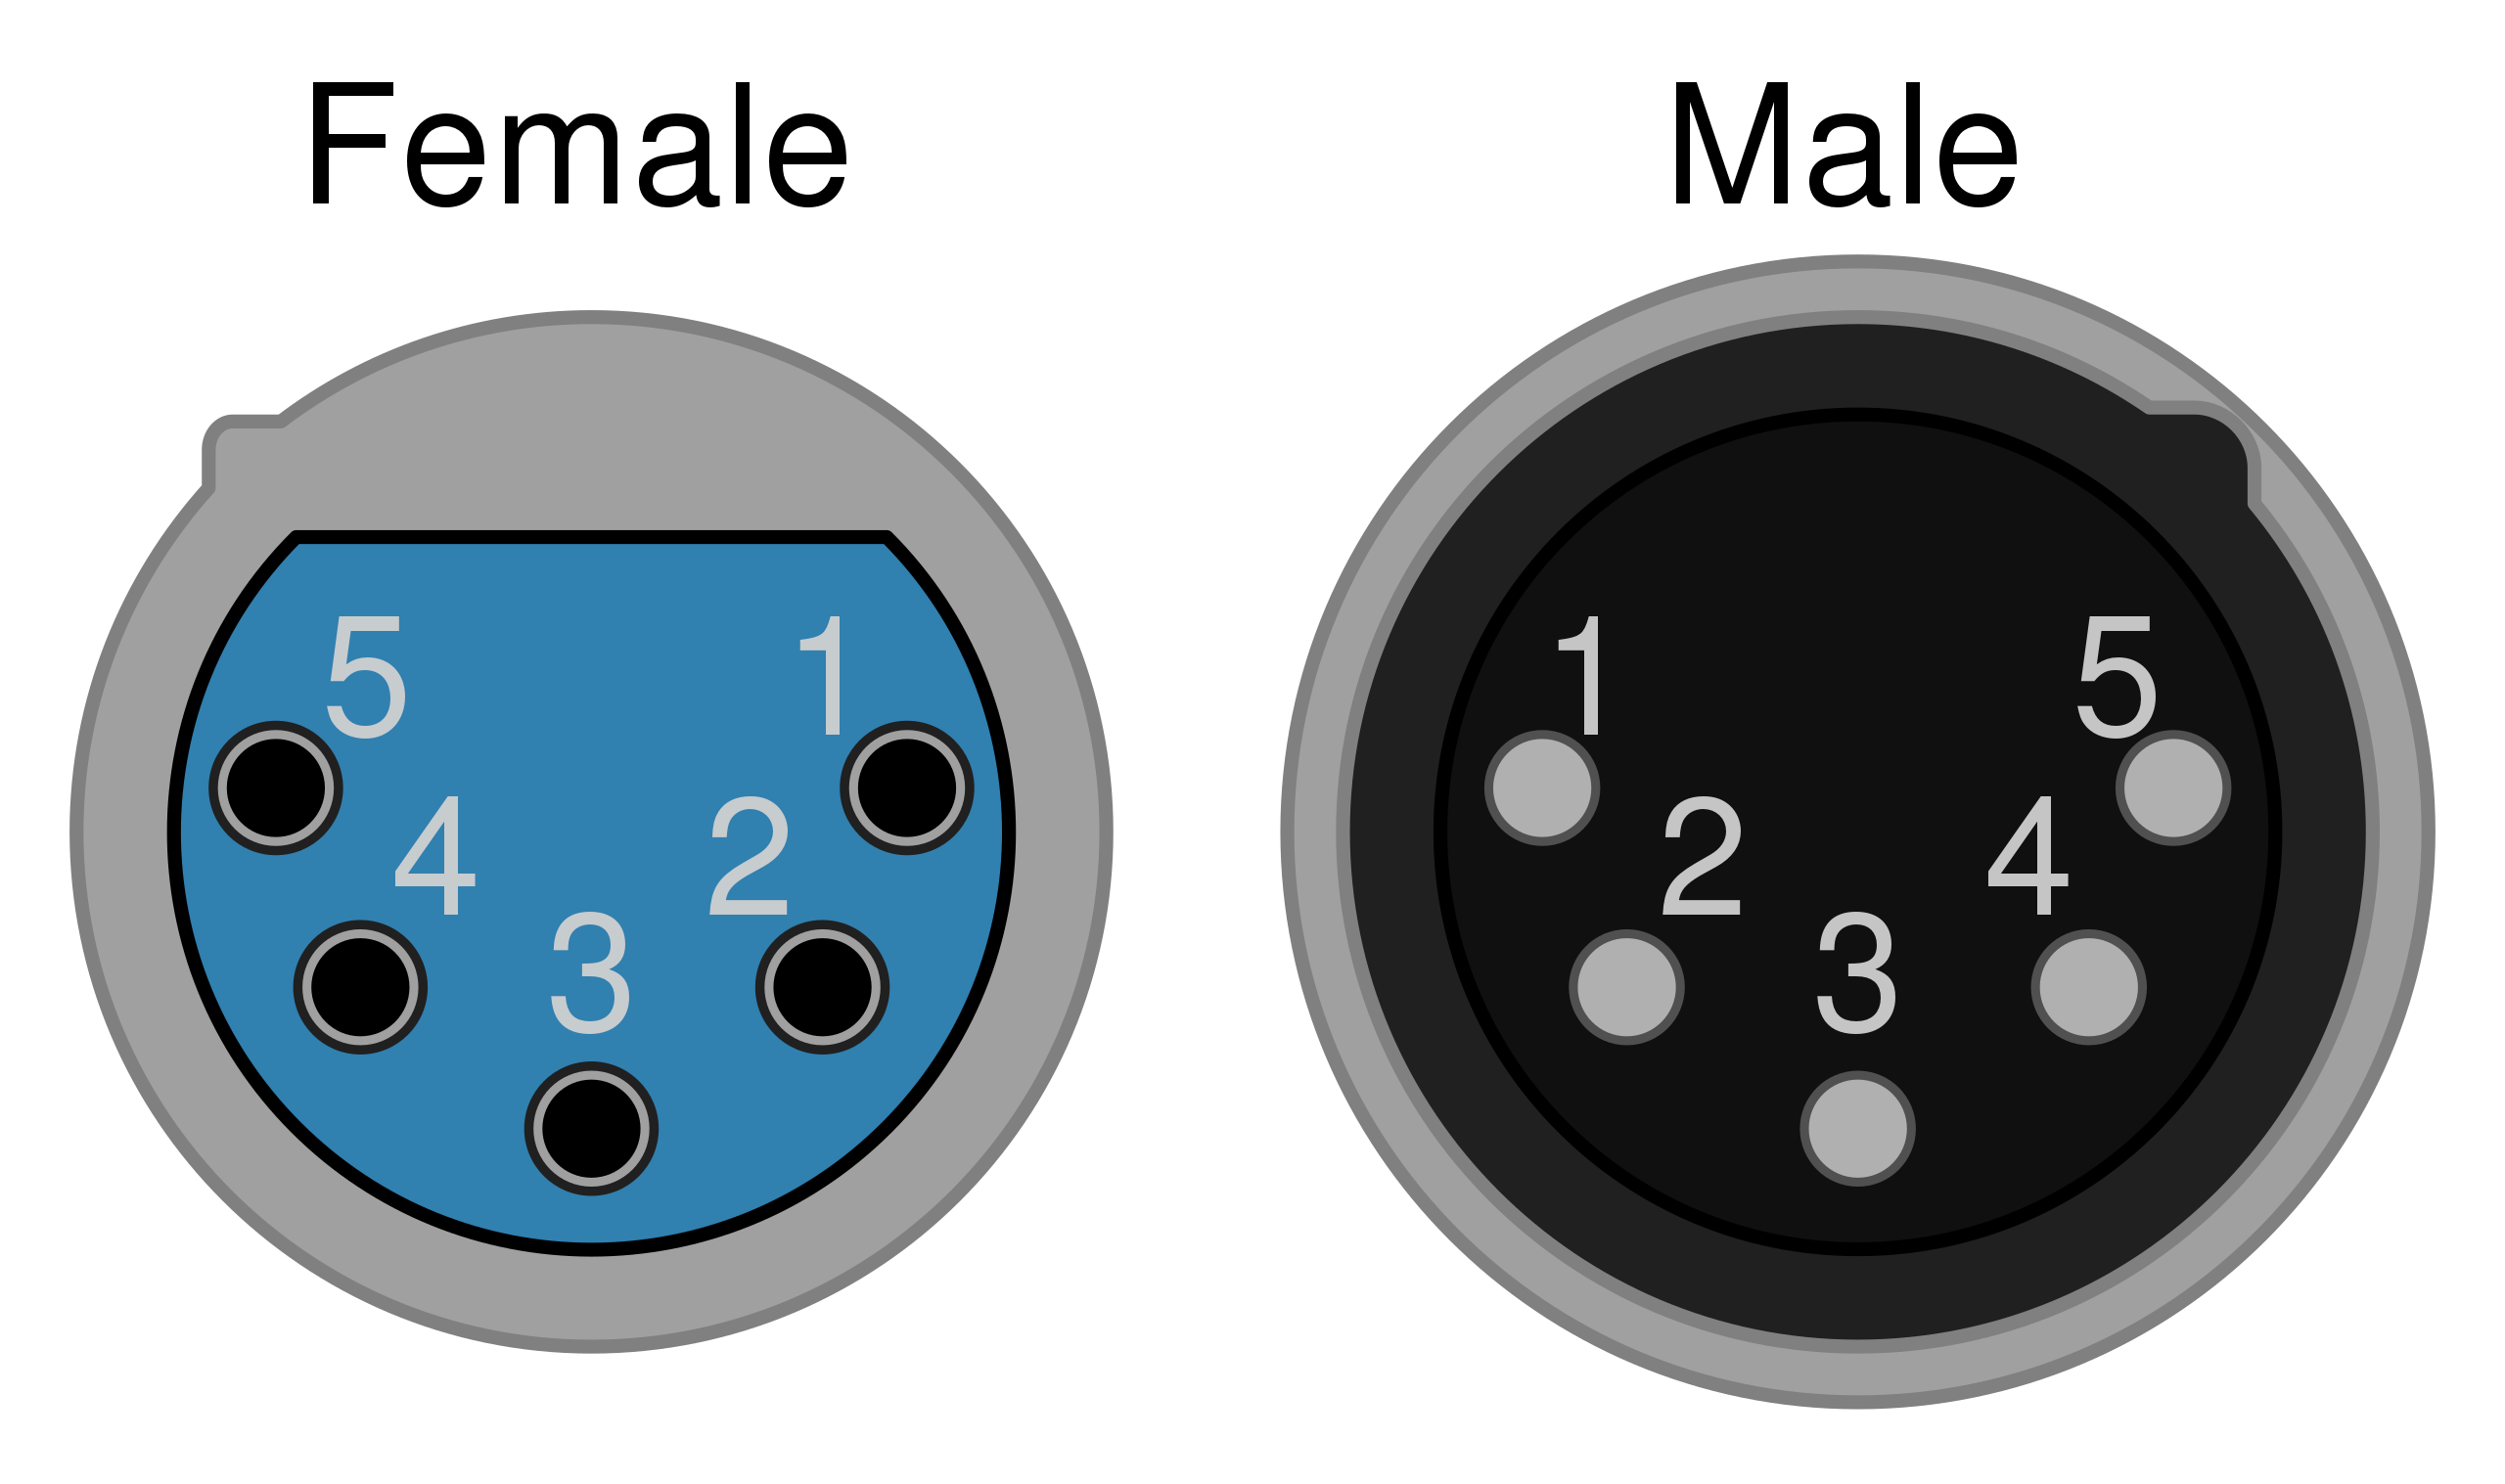
\includegraphics[trim={0 0 0 0.0cm}, clip, scale=0.05]{figures/XLR_stecker.png}
	\caption{XLR5 Pinout - Officialy Used for DMX}
	\label{fig:xlr}
\end{figure}

The endsystems in DMX512 are called fixture because it's most likely a lighting installation which is mounted somewhere.
This could be a moving-head, fresnel, spotlight, stroboscope or any other light installation.
It could also be a fog machine that emits fog on an appropriate signal.

All devices are daisy-chained together visualized in \ref{fig:dmx_diagram}.
The DMX controller is in the beginning of each chain.
The receiving endsystems are chained behind each other from output to input. 
A terminator, specified in the DMX specification, is to be connected to the final output.
 

\begin{figure}[h]
	\centering
	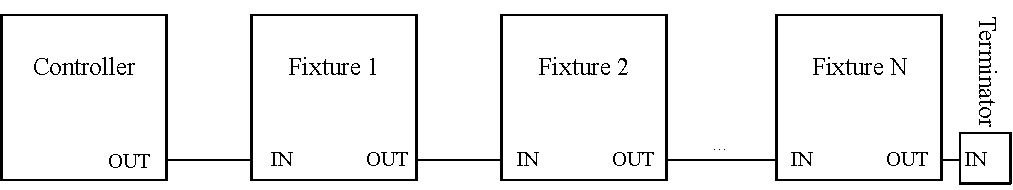
\includegraphics[scale=0.6]{figures/DMX_blockdiagram.pdf}
	\caption{DMX Topology}
	\label{fig:dmx_diagram}
\end{figure}

The hole chain is called DMX-Universe and can contain a set of 512 channels.
If there is a need of more channels one needs more DMX universes - each channel consists of one byte.
Due to the fact that a DMX universe always has its own bus, starting from a new controller can lead to inconveniences.

A channel in the event technology/CAN-Bus is to distinguish between e.g. a Wi-Fi channel.
Each endsystem is assigned at least one but usually several channels.
Every endsystem knows which channel is intended for it, which must be preset.

\begin{figure}[h]
	\centering
	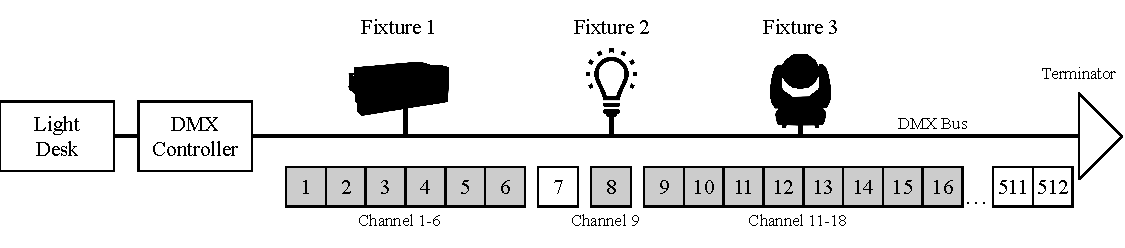
\includegraphics[scale=0.6]{figures/DMX_Chain.pdf}
	\caption{DMX Chain Example}
	\label{fig:dmx_chain}
\end{figure}

In the illustrated example \cref{fig:dmx_chain} the first fixture occupies channels 1-6, while channel 7 is unoccupied.
The second fixture only is a dimmer that can be dimmed in 256 steps, therefore it only needs one channel, the 8th.
The third fixture is a moving head, which occupies channels 9-18 directly behind the dimmer.
The remaining channels are still unoccupied.
The terminator is connected to the end of the DMX bus.
If one byte does not have a high enough resolution, 
merging two bytes to a dual channel of 2 bytes or 65536 different values insted of 256.
E.g., the 360-degree rotation of a moving head is described roughly in the first byte and in fine steps in the other.

Since \ac{DMX} is unidirectional it can be assumed that the endsystems generally only receive or forward (daisy chain) control signals sent from the control console.
This is a major limitation of DMX, beside of the rather small universe size.
It is also not reliable, the use of fire installations is therefore considered too dangerous.

\subsection*{Art-Net}
\label{sec:artnet}
% \begin{itemize}
% 	\item Example of an wifi protocol
% 	\item 2.4 or 5GHz
% 	\item DMX-Like
% 	\item related work
% \end{itemize}

To deal with the limitations of DMX, some further developments have been established, the most common being Art-Net.
Art-Net is a protocol that moves away from the CAN bus and distributes the data via Ethernet in a \ac{LAN}.
The approach remains the same, the individual stations are controlled with a constant update frequency.
There is no longer a limitation of 512 channel universes.
A universe at Art-Net describes 32,768 DMX universes over a single network, far more than is realistically used.
In standard mode, the packets are distributed to the stations with unicasts, by means of connectionless \ac{UDP}.

Because Art-Net is a network protocol, it is also able and designed to distribute packets via WLAN.
The lighting console talks to an \ac{AP} via Ethernet or WLAN 
and this access point forwards the control signals to the individual station.
The choice of WLAN specification is mainly determined by the stations,
so it is just limited to 2.4 GHz or 5 GHz.
Special hardware that supports Art-Net at the factory is expensive
because of the development costs and the relatively low quantities.

\section{ESP Platform}

Almost every 802.11 capable \ac{MCU} could be picked for this research.
But there are several reasons why the ESP Platform from Espressif is a valid choice.
There are several chips provided by Espressif with Wi-Fi specifications, these chips are very affordable
\footnote{3.86 at \url{www.aliexpress.com}, 10.3.2022}
and although the ongoing chip crysis there are still easy to get, in contrast of the also very popular Chips from the manufacturer Arduino, which are also more expansive.
Espressif supports an own development IDF to flash the chips, with minor tweeks it's also to use the Arduino IDE.\\
However, the properitary protocol ESP-Now which, just supported in the ESP Ecosystem, is discussed below
and has promising properties for a solid and fast realisation of a low level protocol.


\subsection*{ESP32 Hardware}

The chip ESP32 is quite common in DIY projects around everything from home automation to light installations 
and can be bought as development boards, which are ready to use.

The chip \ref{fig:esp32} is promoted with several features: 
\footnote{The most recent ESP32 datasheet can be found the documentation page of Espressif, here used: V3.3\\
	\url{https://www.espressif.com/en/support/documents/technical-documents}}
\begin{itemize}
	\setlength\itemsep{-0.0em}
	\item Fast CPU (2 cores at 240 MHz)
	\item 802.11 b/g/n with up to 150 Mbps (2.4GHz)
	\item Wi-fi Multimedia (WMM)
	\item Immediate Block ACK
	\item Automatic Beacon monitoring (hardware TSF)
	\item Virtual Wi-Fi Interfaces
	\item Simultaneous support for Infrastructure, SoftAP, and Promiscuous modes
	\item Bluetooth v4.2 BR/EDR and Bluetooth LE
	\item Advanced Peripheral Interfaces: GPIO, ADC, DAC, touch sensors, hall sensor, 
	SPI, I2S, I2C, UART, CAN, RMT (TX/RX), Motor/LED PWM 
\end{itemize}

\begin{figure}[h]
	\centering
	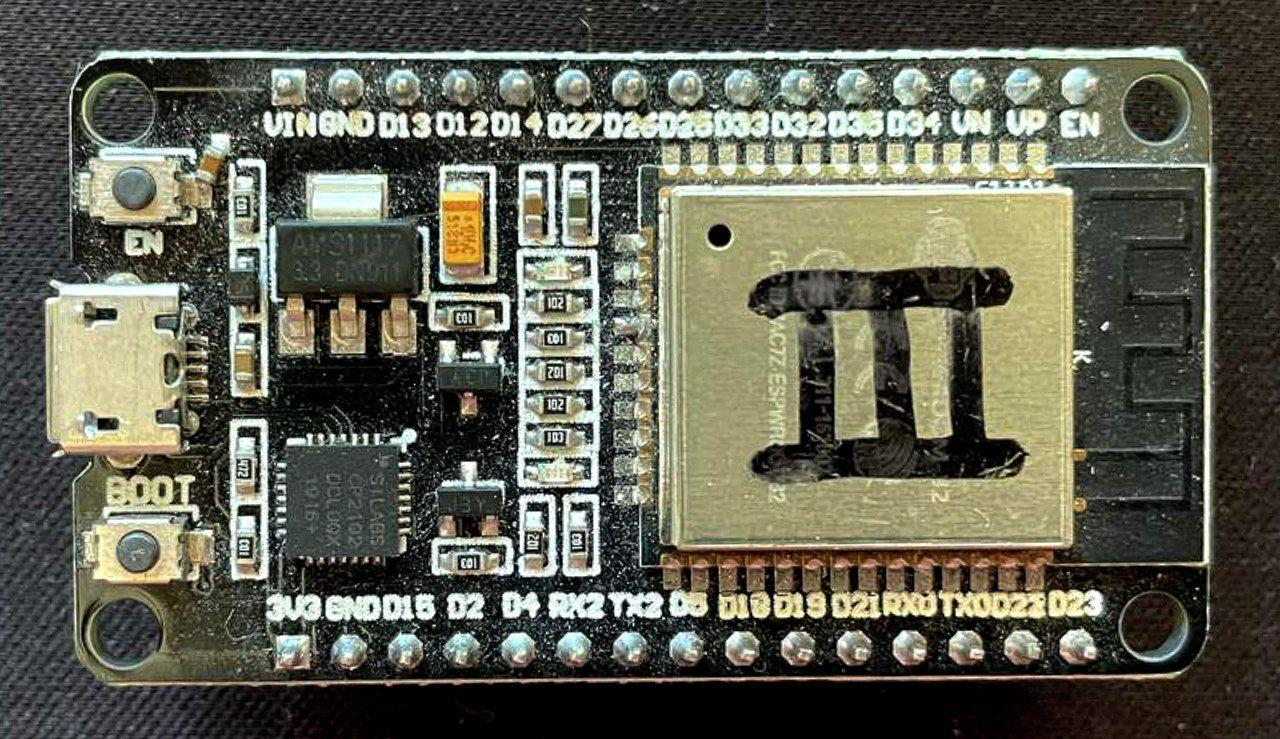
\includegraphics[scale=0.2]{figures/espdevboard.jpg}
	\caption{ESP32 Devboard (Devkit V1)}
	\label{fig:esp32}%
\end{figure}

It can be said that the ESP32 is a low-cost 32-bit microcontroller,
which is quite powerful despite its low power consumption.
The extensive set of features makes it suitable for integration into a wide range of smart environments.
\cite{TheWorkingPrincipalsOfESP32}

\subsection*{ESP-Now}
\label{sub:espnow}
ESP-NOW is a properitary protocol developed by Espressif. 
\emph{ESP-NOW is widely used in smart light, remote controlling, sensor, etc.}
\footnote{\url{https://docs.espressif.com/projects/esp-idf/en/latest/esp32/api-reference/network/esp_now.html}\label{note:espressif}}
It is a connectionless protocol, so the \ac{WES}s are in Ad-Hoc mode instead of \ac{STA}.
It is just supported on the ESP8266, ESP32 and ESP32s, all chipsets from Espressif, but they are compatible with each other.
Because of this, an ESP-Chip is needed as a gateway to interact from the outside to the ESP-NOW communication. 

Through the hardware limitation of the boards it can just be used on the 2.4 GHz frequency band.
ESP-NOW allows 10 ESPs for pairing with encryption and up to 20 without encryption.
Espressif promises throughput of up to 30 MBit/s and a possible range of up to 1 km.
However, Roberto Pasic et al. \cite{ESPNOWCommunication} measured a range of the unmodified onboard antenna of the ESP32 
and just got a \emph{stable communication up to 190 m in open field}.

The focus of the ESP-NOW protocol is on low power consumption.
A connectionless communication between \ac{WES}s not only saves energy during the authentication process, 
Additionally, the commonication is direct and not over an access point, through the properties of ad-hoc networks.
The protocol has a limitation of a limited payload of 250 bytes for each transmission.
It also has much less overhead, which results in shorter airtime, fewer disturbances and also less power consumption through the antenna 
(latter beeing not relevant for this thesis).
There is no TCP/IP header to be transmitted. 
For very small payloads, this offset can become disproportional.

The default ESP-NOW bit rate is 1 Mbps it uses a channel width of 20MHz, 
there is no double channel (40Mbit/s or higher) used.
But e.g., the low energy, 
high range protocol Long Range Wide Area Network (LoRaWAN) suffers from a too slow throuput for this application.

To understand what ESP-NOW does one must take a look to the vendor-specific action frame transmiting ESP-NOW data,
these are Action Frames desinged for vendor-specific signaling.
The compositions of the frame are broken down in more detail in \cref{fig:esp_now_frame_format} and \cref{fig:esp_now_vendor_format}
\footnote{\url{https://docs.espressif.com/projects/esp-idf/en/latest/esp32/api-reference/network/esp_now.html}}

\begin{table}[h]
	\centering
	\begin{tblr}{	hlines,
					vlines,
					rows = {ht=1.3cm},
					columns = {halign=c},
					colspec = {XXXXXX},} 
	\makecell{MAC\\Header} & \makecell{Category\\Code} & \makecell{Org.} & 
	\makecell{Random\\Values} & \makecell{Vendor\\Specific\\Content} & \makecell{FCS}\\
	\end{tblr}
	\begin{tabularx}{\linewidth}{ X X X X X X }
		\makecell{\footnotesize{24}} & \makecell{\footnotesize{1}} & \makecell{\footnotesize{3}} & 
		\makecell{\footnotesize{4}} & \makecell{\footnotesize{7 $\sim$ 255}} & \makecell{\footnotesize{4}} \\
	\end{tabularx}
	\caption{ESP-NOW Frame Format}
	\label{fig:esp_now_frame_format}
\end{table}

\todo{Check out at the end, if formatation is broken}
\begin{itemize}
	\setlength\itemsep{-0.0em}
	\item \textbf{MAC Header:} As ESP-NOW is connectionless, the MAC header differs from that of standard frames.
	\item \textbf{Category Code:} The Category Code field is set to the value(127) indicating the vendor-specific category.
	\item \textbf{Organization Identifier:} The Organization Identifier contains a unique identifier (0×18fe34), which is the first three bytes of MAC address applied by Espressif.
	\item \textbf{Random Value:} The Random Value field is used to prevent relay attacks.
	\item \textbf{Vendor Specific Content:} The Vendor Specific Content contains vendor-specific fields (table \ref{fig:esp_now_vendor_format})
	\item \textbf{Frame Check Sequence:} Used for error correction in layer 2.
\end{itemize}

\newpage

\begin{table}[h]
	\begin{tblr}{	hlines,
					vlines,
					rows = {ht=1.3cm},
					columns = {halign=c},
					colspec = {XXXXXX},} 
		\makecell{Element\\ID}& \makecell{Length} & \makecell{Org.\\Identifier} & \makecell{Type} & \makecell{Version} & \makecell{Body}  \\
	\end{tblr}
	\begin{tabularx}{\linewidth}{ X X X X X X }
		\makecell{\footnotesize{1}} & \makecell{\footnotesize{1}} & \makecell{\footnotesize{3}} & \makecell{\footnotesize{1}} & \makecell{\footnotesize{4}} & \makecell{\footnotesize{7 $\sim$ 250}} \\
	\end{tabularx}

	\caption{Vendor Specific Content}
	\label{fig:esp_now_vendor_format}
\end{table} 

\begin{itemize}
	\setlength\itemsep{-0.0em}
	\item \textbf{Element ID:} The Element ID field is set to the value (221), indicating the vendor-specific element.
	\item \textbf{Length:} The length is the total length of Organization Identifier, Type, Version and Body.
	\item \textbf{Organization Identifier:} The Organization Identifier contains a unique identifier(0×18fe34), which is the first three bytes of MAC address applied by Espressif.
	\item \textbf{Type:} The Type field is set to the value (4) indicating ESP-NOW.
	\item \textbf{Version:} The Version field is set to the version of ESP-NOW.
	\item \textbf{Body:} The Body contains the ESP-NOW data.
\end{itemize}

It is worth to mention, that the vendor specific content (\ref{fig:esp_now_frame_format}) is allowed to contain up to 255 bytes.
But the sum over all values (\ref{fig:esp_now_vendor_format}), if the body would contain the maximum of 250 bytes, 
leads to a total of 260 bytes.
The values are from the documentation of ESP-NOW from Espressif.
They also claim in the ESP-NOW documentation, that broadcast is not supported, but it is.
It seems that the documentation
\footnote{\url{https://docs.espressif.com/projects/esp-idf/en/latest/esp32/api-reference/network/esp_now.html}}
isn't completely finished (or translated).